\chapter{Antecedentes generales y propuesta} % Título del capítulo. Lo agrega automaticamente al índice.
\label{cap:antecedentes} % etiqueta para las referencias a este capítulo
\markboth{Antecedentes generales y propuesta}{Antecedentes generales y propuesta} % Título que aparecerá en la cabecera de las siguientes páginas.
\vspace*{-2cm} % Reduce el espaciado, para que el parrafo este mas cerca del título.


% Descripción detallada del problema.
% Estado del arte: formas de abordar el problema (teorías, métodos, etc.).
% Solución propuesta en base a lo presentado en el estado del arte.


%\lipsum[1-5]
%paper 1: \cite{taigman_unsupervised_2016} \\
%\cite{goodfellow_generative_2014}
%\cite[papqwqweasdasder]{bauGANDissectionVisualizing2018}
\section{Planteamiento del problema}
Las GANs es un nuevo tipo de arquitectura dentro del Machine Learning propuesta el 2014 por Ian Goodfellow \cite{goodfellowGenerativeAdversarialNetworks2014}
en donde dos redes neuronales compiten entre si, generalmente con el objetivo de sintetizar o crear datos.
Esta arquitectura a tenido gran aceptación en el campo de la Visión por Computador debido a los buenos resultados que muestra
para sintetizar imágenes. Estas dos redes neuronales cuando ya están entrenadas, generan un modelo de Machine Learning capaz de ejecutarse
y generar síntesis de imágenes, pero para hacerlo debe de implementarse en alguna parte. Esta implementación puede ser costosa y muchas veces
una razón para que un estudio o investigación nunca llegue a implementarse.

En la actualidad, es un tópico del Deep Learning pocas veces incluido o dictado  en la enseñanza
debido a la escasa información disponible sobre el funcionamiento de estos modelos en el idioma español, no existiendo una plataforma que muestre este contenido, ejemplos e implementación del modelo corriente en tiempo real.
Además, TensorFlow.js es una API dentro de todo el ecosistema de TensorFlow que lleva poco
más de un año en su versión estable 2.0, que posee sus propias herramientas de visualización que hacen uso de toda la potencia del desarrollo web, por lo que una implementación de una primera plataforma de aprendizaje web en español utilizando esta herramienta sería una elección bastante acertada.


%Esto lleva al estudio de los requerimientos necesarios para su ejecución y sintonización
%en un nuevo tipo de framework.
\clearpage
\section{Solución a la problemática}
El presente proyecto busca desarrollar e implementar un sistema capaz de ejecutar una red neuronal de tipo GAN de forma online, haciendo de la implementación del modelo lo más simple posible para facilitar su estudio y posterior extensión a otros modelos, embebiendo este sistema en una plataforma didáctica online que ayude, facilite y acelere la comprensión y el estudio de estos modelos más complejos.

Para esto, la plataforma debe de contar con una interfaz gráfica que permita la selección de los modelos, para posteriormente mostrar en la página de cada uno tres secciones relacionadas a este: una sección de ejecución del modelo directamente en el navegador, una sección de visualización de entrenamiento si la carga del modelo lo permite,  y una última sección en donde se describa al modelo en cuanto a su funcionamiento y procesos, además de su propia implementación en TensorFlow.js .

\begin{figure}[h]
  \includegraphics[scale=0.7]{img/fix0/diag_plataforma}
  \centering
  %\vspace{-0.1cm}
  \caption{Funcionamiento básico plataforma propuesta}
  \label{fig:diag_plataforma}
\end{figure}



\clearpage
\section{Objetivos}
%\addcontentsline{toc}{section}{Objetivos generales}

\subsubsection{Objetivo General}
\begin{itemize}
\item     Desarrollar e implementar una plataforma de enseñanza disponible en línea para redes generativas GAN.
\end{itemize}

\subsubsection{Objetivos Específicos}
%\addcontentsline{toc}{section}{Objetivos generales}
\begin{itemize}
\item Estudiar la arquitectura GAN y su funcionamiento.
\item Estudiar los lenguajes de desarrollo web, especialmente los de Frontend como JavaScript.
\item Investigar y estudiar acerca del ecosistema de desarrollo web en Machine Learning, y determinar las limitaciones de este ecosistema.
\item Elaborar un marco de desarrollo en un ambiente Python - JavaScript.
\item Implementar posibles soluciones existentes de ejecución de redes neuronales a nivel local, para posteriormente hacerlo en línea.
\item Lanzar a plataforma online para su evaluación.

%\item Investigación de la literatura existente sobre GAN, fundamentos del Deep Learning y frameworks de ML.
%\item Implementar posibles soluciones existentes de ejecución de redes neuronales a nivel local.
%\item Diseñar e implementar un sistema capaz de ejecutar redes neuronales basadas en GAN.
\end{itemize}
%\subsection{Frameworks: TensorFlow.JS
%\subsection{Propuesta de solución}

\clearpage
\section{La Inteligencia Artificial y el Aprendizaje Automático}

La Inteligencia Artificial o IA, es un campo de investigación y estudio
que intenta comprender \emph{cómo los seres humanos pensamos} y construir
a partir de esto entidades o máquinas que muestren capacidades cognitivas,
que perciban, entiendan, infieran o deduzcan, es decir, que demuestren
\emph{inteligencia}.

El Aprendizaje Automático o Machine Learning, es un subcampo de la Inteligencia Artificial,
que intenta dotar a una máquina o sistema con la capacidad de aprender de datos sin
haber sido explícitamente programada. Para esto se desarrollan
algorítmos con la capacidad de generalizar comportamientos
y aprender patrones, y de esta forma mejorar, describir y predecir ciertos resultados.

\begin{figure}[h]
    \includegraphics[scale=0.4]{img/1}
    \centering
    %\vspace{-0.1cm}
    \caption{Inteligencia Artificial, Aprendizaje Automático y Deep Learning \cite{cholletDeepLearningPython2018a}}
    \label{1}
\end{figure}

En general, las técnica o enfoques del Machine Learning se pueden dividir en 3
categorías:
\begin{itemize}
  \item \textbf{Aprendizaje Supervisado (\emph{Supervised Learning}):} al sistema o máquina se le presenta
  un conjunto de datos o ejemplos de entrenamiento, compuestos por los valores de entrada
  y los valores de salida deseados. A partir de ello se busca generalizar un patrón
  mediante algún algorítmo para hacer predicciones conocidas y posibles sin conocer.

  \item \textbf{Aprendizaje No Supervisado (\emph{Unsupervised Learning}):} el sistema se dota
  de un conjunto de entrenamiento compuesto sólo por los valores de entrada, sin los valores de
  salida deseados. Es decir, el conjunto de entrenamiento no contiene los resultados
  debidamente etiquetas, clasificados o categorizados para cada uno de los valores de entrada,
  por lo que el algorítmo debe aprender a realizar la clasificación o categorización
  de los datos sólo a partir de los valores de entrada.

  \item \textbf{Aprendizaje por Refuerzo (\emph{Reinforcement Learning}):} el sistema
  o máquina a través de la interacción aprende lo bueno o malo de una acción a través
  del resultado obtenido. Si la acción o comportamiento es el correcto, la recompensa
  es positiva, en caso contrario, la recompensa será negativa.
\end{itemize}

%%%%%%%%%%%%%%%%%%%%%%%%%%%%%%%%%%%%%%%%%%%%%%%%%%%%%%%%%%%%%%%%%%%%%%%%%%%%%%%
%%%%%%%%%%%%%%%%%%%%%%%%%%%%%%%%%%%%%%%%%%%%%%%%%%%%%%%%%%%%%%%%%%%%%%%%%%%%%%%
%%%%%%%%%%%%%%%%%%%%%%%%%%%%%%%%%%%%%%%%%%%%%%%%%%%%%%%%%%%%%%%%%%%%%%%%%%%%%%%
%%%%%%%%%%%%%%%%%%%%%%%%%%%%%%%%%%%%%%%%%%%%%%%%%%%%%%%%%%%%%%%%%%%%%%%%%%%%%%%
%%%%%%%%%%%%%%%%%%%%%%%%%%%%%%%%%%%%%%%%%%%%%%%%%%%%%%%%%%%%%%%%%%%%%%%%%%%%%%%
%%%%%%%%%%%%%%%%%%%%%%%%%%%%%%%%%%%%%%%%%%%%%%%%%%%%%%%%%%%%%%%%%%%%%%%%%%%%%%%

\section{El Deep Learning}

El Deep Learning o Aprendizaje Profundo, es un subcampo del Machine Learning que utiliza como arquitectura fundamental
\emph{Redes Neuronales}. Utiliza este tipo de redes como forma para extraer información de los datos con el menor esfuerzo
humano posible, intentando hacer el proceso de forma automática.\\
Gran parte de los conceptos básicos del Deep Learning surgieron en los años 60, 80 y 90, pero ha tenido su mayor auge en la última
decada debido principalmente a factores como la digitalización de la información y la consiguiente habilidad de acceder a datos
fácilmente, haciendo que muchos problemas tengan ahora una forma digital. Comunidades científicas que debido al avance de las
telecomunicaciones y en especial el internet, son capaces de trabajar y compartir remotamente. Grandes avances en la computación
y el diseño de nuevo Hardware (CPU, GPU, TPU), permitiendo la ejecución efectiva a gran escala. Desarrollo de herramientas
como TensorFlow, PyTorch y Keras con grandes niveles de abstracción que ayudan a las personas a resolver
problemas en cada vez menos tiempo y con cada vez menos conocimientos, dejando a la ``idea'' y los ``datos'' como el punto central
y no el esfuerzo.

Para esto, utiliza un conjunto de datos de ejemplo como \textbf{base o set de entrenamiento} que se utiliza para reconocer
patrones. Una vez que se extraen estos patrones, el sistema puede ser capáz de utilizarlos para \emph{etiquetar} nuevos
datos de entrada.\\



%\begin{figure}[h]
 %   \includegraphics[scale=0.3]{img/5}
 %   \centering
    %\vspace{-0.1cm}
 %   \caption{Capas de una red neuronal}
 %   \label{5}
%\end{figure}


%%%%%%%%%%%%%%%%%%%%%%%%%%%%%%%%%%%%%%%%%%%%%%%%%%%%%%%%%%%%%%%%%%%%%%%%%%%%%%%
%%%%%%%%%%%%%%%%%%%%%%%%%%%%%%%%%%%%%%%%%%%%%%%%%%%%%%%%%%%%%%%%%%%%%%%%%%%%%%%
%%%%%%%%%%%%%%%%%%%%%%%%%%%%%%%%%%%%%%%%%%%%%%%%%%%%%%%%%%%%%%%%%%%%%%%%%%%%%%%
%%%%%%%%%%%%%%%%%%%%%%%%%%%%%%%%%%%%%%%%%%%%%%%%%%%%%%%%%%%%%%%%%%%%%%%%%%%%%%%
%%%%%%%%%%%%%%%%%%%%%%%%%%%%%%%%%%%%%%%%%%%%%%%%%%%%%%%%%%%%%%%%%%%%%%%%%%%%%%%
%%%%%%%%%%%%%%%%%%%%%%%%%%%%%%%%%%%%%%%%%%%%%%%%%%%%%%%%%%%%%%%%%%%%%%%%%%%%%%%

\subsection{Estructura de las Redes Neuronales}

Las redes neuronales están compuestas por capas, y cada una de estas capas está compuesta por nodos o neuronas.
Los nodos tienen la siguiente estructura:
\begin{itemize}
    \item Una o más entradas que reciben los datos a procesar.
    \item Pesos dados a cada una de las entradas. Estos aumentan o disminuyen la importancia de dicha entrada.
    \item Función sumatoria, encargada de sumar todas las combinaciones de peso-entrada.
    \item Función de activación, que determina la activación o no de un nodo según el valor obtenido en la Función sumatoria.
            Esta función puede ser una simple función escalón, una función lineal que devuelve el mismo valor calculado, una
            función lineal por tramos que devuelve un valor si el valor de la función sumatoria está dentro de ciertos límites
            como la función ReLU.
\end{itemize}

\begin{figure}[H]
    \includegraphics[scale=0.4]{img/4}
    \centering
    %\vspace{-0.1cm}
    \caption{Estructura de una neurona}
    \label{4}
\end{figure}

\begin{figure}[H]
    \includegraphics[scale=0.6]{img/5}
    \centering
    %\vspace{-0.1cm}
    \caption{Capas de una red neuronal}
    \label{5}
\end{figure}


Para entender el modelo de redes neuronales, se deben definir los siguientes concepto básicos:
\begin{itemize}
    \item \textbf{Etiquetas:} tambień llamadas \emph{labels} por su nombre en inglés. Corresponde al valor, clasificación
            o categoría a predecir.
    \item \textbf{Atributos:} también llamados \emph{features}. Corresponden a las variables de entrada a cada nodo o neurona.
    \item \textbf{Set de datos:} corresponde a los ejemplos a utilizar para entrenar o hacer predicciones con el modelo.\\
                Estos ejemplos pueden corresponder a atributos debidamente etiquetados, que suelen utilizarse como ejemplos de
                entrenamiento para un modelo, o pueden corresponder a atributos sin etiquetar que se utilizan para probar
                el modelo ya entrenado o en instancias de aprendizaje no supervisado.
\end{itemize}


\clearpage
\subsection{Entrenamiento de una red neuronal}

Con el fin de extraer información de los datos, el modelo de red neuronal debe definir la relación entre las entradas o atributos
y su salida o etiquetas. Para esto el modelo debe pasar por el proceso de entrenamiento o aprendizaje para posteriormente
poder hacer inferencias de acuerdo a los patrones aprendidos durante el entrenamiento.

En el \textbf{proceso de entrenamiento} ocurre un ajuste o modificación de los pesos asociados a cada entrada a un nodo,
con el fin de minimizar un \emph{función de pérdida}. Esta \emph{Función de Pérdida} recibe la predicción \emph{\^y} y la
etiqueta correcta \emph{y}, asociadas a ciertos atributos. Con esto, la \emph{Función de Pérdida} calcula lo incorrecto
o no de una predicción. \\
Estas \emph{Funciones de Pérdida o Costo} pueden eliguirse de acuerdo al tipo de modelo de red neuronal a implementar
para evaluar su rendimiento o performance. Entre estas, una de las más utilizadas es la MSE, Mean Square Error, también conocida
como \emph{Costo cuadrático}, definida como:
\begin{equation}
    MSE = \frac{1}{N}
        \sum (y - (prediccion(x)))^2
\end{equation}

Los pesos se suelen inicializar con valores escogidos de forma aleatoria, y generalmente
son números pequeños. El ajuste de estos pesos ocurre gracias a un algorítmo de optimización,
que ayudan a reducir o minimizar la \emph{Función de Pérdida}. Estos algorítmos de optimización suelen estar
basados en el cálculo del \textbf{gradiente} de la \emph{función de pérdida}, debido a que éste indica la dirección de
máximo crecimiento de la función en cierto punto. Este tipo de algorítmos es por tanto llamado
 \textbf{Descenso de Gradiente}, y son técnicas conocidas como \textbf{Gradient Descent Optimization}. Entre ellas
 se encuentran una gran variedad de algorítmos que implementan el Descenso de Gradiente, tales como Adagrad, Adadelta,
 Adam, Adamax, Nadam, y otros \cite{ruderOverviewGradientDescent2017}.

 Para actualizar el peso una vez que la \emph{Función de Pérdida} a calculado el error y el algorítmo de optimización
 a recalculado los pesos para \emph{minimizar la Función de Pérdida}, se recurre a un algorítmo de propagación hacia atras,
 desde la capa de salida hacia las capas anteriores. Este algorítmo de propagación se conoce como \textbf{Backpropagation}
 o \textbf{Propagación hacia atras} \cite{gershensonArtificialNeuralNetworks2003} \cite{epelbaumDeepLearningTechnical2017}.


\clearpage
\subsection{Breve historia de la IA y el Deep Learning}
La Inteligencia Artificial, y más específicamente, el Deep Learning, a
pesar de que suelen parecer temas nuevos de investigación y estudio, están basado en ideas
de los años 60, 80 y 90.\\
A pesar de que se puede pensar que son descubrimientos recientes, es un campo
que ha tenido una lenta y gradual evolución a través de varias decadas. A continuación se presenta
un resumen no exhaustivo de parte de los grandes hitos en el desarrollo del \emph{Deep Learning}.



\begin{itemize}
    \item \textbf{1943:} Warren S. McCulloch y Walter Pitts llevan el modelo conocido de la neuronas
            a la matemática, mostrando con esto el primero modelo matemático de la neurona biológica. \cite{mccullochLogicalCalculusIdeas1943} \\

    \item \textbf{1957:} Frank F. Rosenblatt basandose en el modelo matemático propuesto por Pitts y McCulloch,
            propone la idea del \emph{Perceptron}, una red neuronal de una sola capa capaz de
            realizar clasificación binaria. Un par de años más tarde (1962) propone también la idea
            de una red de múltiples capas. \cite{rosenblattPerceptronProbabilisticModel1958} \\

    \item \textbf{1960:} Henry J. Kelley muestra por primera vez un modelo de propagación hacia atrás o
    Backpropagation en el contexto de la Teoría de Control. \cite{kelleyGradientTheoryOptimal1960} \\

    \item \textbf{1962:} Stuart Dreyfus demuestra un modelo de Backpropagation que funciona utilizando
        simples derivadas y la regla de la cadena. \cite{dreyfusNumericalSolutionVariational1962} \\


    \item \textbf{1965:} Alexey Grigoryevich Ivakhnenko y Valentin Grigorevich Lapa crean el
    primer algorítmo de aprendizaje para el entrenamiento de perceptrones multicapa, utilizando entrenamiento
    GMDH (Group Method of Data Handling o Método de agrupamiento para el manejo de datos) y funciones
    de activación polinomial. Son considerador por esto como los padres del \emph{Deep Learning}. \cite{ivakhnenkoCyberneticPredictingDevices1966} \\

    \item \textbf{1970:} Seppo Linnainmaa presenta en su tesis de Master y en un artículo posterior
            el primer código de diferenciación automática y Backpropagation.  \cite{linnainmaaTaylorExpansionAccumulated1976} \\

    \item \textbf{1980:} Kunihiko Fukushima inventa las Convolutional Neural Network (CNN) al proponer
    su arquitectura \emph{Neocognitron} capaz de reconocer patrones visuales. \cite{fukushimaNeocognitronSelforganizingNeural1980}\\


    \item \textbf{1982:} John Hopfield crea la primera arquitectura reconocida como una Recurrent Neural Network (RNN).
            Esta misma sería conocida más tarde como \emph{Hopfield Network}, siendo fundamental
            para los modelos posteriores de RNN. \cite{hopfieldNeuralNetworksPhysical1982}\\

    \item \textbf{1985:} David H.Ackley, Geoffrey E.Hinton y Terrence J.Sejnowski crean la Boltzmann Machine,
    una especie de RNN estocástica sin capa de salida. \cite{ackleyLearningAlgorithmBoltzmann1985}\\


    \item \textbf{1986:} David E. Rumelhart, Geoffrey E. Hinton y Ronald J. Williams muestran la primera implementación
        exitosa del algorítmo de Backpropagation en el entrenamiento de las redes neuronales.
    \cite{rumelhartLearningRepresentationsBackpropagating1986}\\
    %\item \textbf{1986:} RBM
    \item \textbf{1989:} Yann LeCun muestra la primera implementación del algorítmo de Backpropagation
    en el entrenamiento de Convolutional Neural Network.\cite{lecunBackpropagationAppliedHandwritten1989}\\

    \item \textbf{1997:} Sepp Hochreiter and Jürgen Schmidhuber proponen la arquitectura Long Short-Term Memory (LSTM), una
    arquitectura de red tipo RNN con conexiones del tipo \emph{feedback} que le permiten procesar secuencias
    de datos. \cite{hochreiterLongShortTermMemory1997}\\

    \item \textbf{2006:} Geoffrey E. Hinton, Simon Osindero y Yee Whye Teh crean la Deep Belief Network y
    mejoran el proceso de entrenamiento haciendolo más eficiente. Se comienza a utilizar el término \emph{Deep Learning}
    con la connotación que hoy se conoce. \cite{hintonFastLearningAlgorithm2006}\\


    \item \textbf{2009:} Fei-Fei Li lanza ImageNet. Base de datos de más de 14 millones de imágenes y más de 20000
    categorías debidamente etiquetadas.\\

    \item \textbf{2012:} Alex Krizhevsky presenta AlexNet en NIPS, un modelo o arquitectura que implementa Convolutional Neural
    Networks mediante GPU, alcanzado una capacidad en la clasificación de imágenes de ImageNet nunca antes vista. \cite{krizhevskyImageNetClassificationDeep2012}\\

    \item \textbf{2014:} Ian Goodfellow propone las Generative Adversarial Network, conocidas como GAN. Con ello
    se abre la puerta a la aplicación de generación de imagénes y video debido a su gran capacidad de sintetizar datos. \cite{goodfellowGenerativeAdversarialNetworks2014}
\end{itemize}

Para un cuadro más exhaustivo de la historia de la IA y el Deep Learning, se sugiere revisar el árticulo
``Deep Learning in Neural Networks: An Overview'' por Juergen Schmidhuber \cite{schmidhuberDeepLearningNeural2015}, en el que
intenta hacer una recopilación de cada una las personas que han contribuido al desarrollo del Deep Learning.


%%%%%%%%%%%%%%%%%%%%%%%%%%%%%%%%%%%%%%%%%%%%%%%%%%%%%%%%%%%%%%%%%%%%%%%%%%
%%%%%%%%%%%%%%%%%%%%%%%%%%%%%%%%%%%%%%%%%%%%%%%%%%%%%%%%%%%%%%%%%%%%%%%%%%
%%%%%%%%%%%%%%%%%%%%%%%%%%%%%%%%%%%%%%%%%%%%%%%%%%%%%%%%%%%%%%%%%%%%%%%%%%
%%%%%%%%%%%%%%%%%%%%%%%%%%%%%%%%%%%%%%%%%%%%%%%%%%%%%%%%%%%%%%%%%%%%%%%%%%
%%%%%%%%%%%%%%%%%%%%%%%%%%%%%%%%%%%%%%%%%%%%%%%%%%%%%%%%%%%%%%%%%%%%%%%%%%
%%%%%%%%%%%%%%%%%%%%%%%%%%%%%%%%%%%%%%%%%%%%%%%%%%%%%%%%%%%%%%%%%%%%%%%%%%

\clearpage
\section{GANs: Generative Adversarial Networks}

Las Redes Generativas Adversariales, o GANs, fueron descritas por primera vez el 2014 en el artículo de Ian Goodfellow
``Generative Adversarial Networks'' \cite{goodfellowGenerativeAdversarialNetworks2014}. Son una clase dentro de las técnicas
del Machine Learning que permiten la generación de imagénes sintéticas, forzando las imágenes sintéticas generadas a ser
estadísticamente indistinguibles de las imágenes originales. La gran capacidad de generación y la potencia de la idea de las redes
adversariales generativas ha hecho que en los últimos años se haya puesto el foco en su investigación y en la generación de nuevas
arquitecturas \cite{panRecentProgressGenerative2019}\cite{wangGenerativeAdversarialNetworks2019} \cite{gujarGenerativeAdversarialNetworks2019}.\\

\begin{figure}[H]
    \includegraphics[scale=0.3]{img/2}
    \centering
    %\vspace{-0.1cm}
    \caption{GANs y su relación en el campo de la Inteligencia Artificial \cite{langrGANsActionDeep2019}}
    \label{2}
\end{figure}

Las GANs consisten básicamente en dos redes que compiten mutuamente: una \textbf{red genera datos falsos}, y la otra \textbf{intenta
distinguir los datos falsos de los reales}.\\
De esta forma, las GANs:
\begin{itemize}
    \item  Es un modelo \emph{generativo} porque tiene como proposito el generar nuevos datos.
    \item Son \emph{redes}
    porque fundamentalmente la arquitectura está compuesta de dos redes neuronales; Discriminador y Generador.
    \item Son
    \emph{adversarias o antagónicas} debido a que el Discriminador compite con el Generador
\end{itemize}

\clearpage
\subsection{Funcionamiento de las GANs}

Las GANs constan en su forma más básica de dos redes neuronales, \emph{Generador} y \emph{Discriminador}. De acuerdo a lo anterior,
los aspectos básicos y fundamentales de estas redes son:
\vspace{-0.6cm}

\subsubsection{Generador}
\vspace{-0.4cm}
\begin{itemize}
    \item Tiene como \textbf{entrada} un vector de números aleatorios, seleccionado de un espacio latente predefinido, como una función normal
        multivariada.
    \item La \textbf{salida} es un ejemplo sintetizado falso que intenta ser estadísticamente lo más parecido a un ejemplo real.
    \item El \textbf{objetivo} es generar datos falsos que sean indistinguibles de los datos reales.
\end{itemize}

\vspace{-0.6cm}
\subsubsection{Discriminador}
\vspace{-0.4cm}
\begin{itemize}
    \item Tiene como \textbf{entradas}:
    \begin{itemize}
        \item Los datos reales, que provienen de la base de datos de entrenamiento.
        \item Los datos falsos, sintetizados por el Discriminador.
    \end{itemize}
    \item La \textbf{salida} es la probabilidad del ejemplo en la entrada de ser real.
    \item El \textbf{objetivo} es distinguir los datos falsos provenientes del Generador y los datos reales
        de la base de datos.
\end{itemize}

\begin{figure}[H]
    \includegraphics[scale=0.25]{img/3}
    \centering
    %\vspace{-0.1cm}
    \caption{Interacción y funcionamiento de las GANs \cite{langrGANsActionDeep2019}}
    \label{3}
\end{figure}

\begin{enumerate}
    \item \textbf{Conjunto de entrenamiento:} Base de datos de ejemplos reales. El Generador debe aprender a emular de forma
                                              perfecta estos datos. Estos datos sirven como entrada a la red Discriminador.
    \item \textbf{Vecto de ruido aleatorio:} Vector/dato \textbf{z} de entrada a la red Generador. Esta entrada es utilizada
                                            por el Generador como punto de partida para la síntesis de datos falsos.
    \item \textbf{Red Generadora:} Toma como entrada un vector de números aleatorio \textbf{z}, y genera como salida un dato
                                    falso \textbf{x*}. El objetivo es que el dato falso sea indistinguible del dato real.
    \item \textbf{Red Discriminadora:} Toma como entrada un dato real \textbf{x} o un dato falso \textbf{x*}. El objetivo
                                        es determinar, para cada dato, la probabilidad si es real.
    \item \textbf{Proceso iterativo de entrenamiento/sintonización:} Para cada una de las predicciones del Discriminador,
                se determina lo buena o no de esta, y se utiliza el resultado para volver a sintonizar la red Discriminadora
                y Generadora mediante Backpropagation.
\end{enumerate}





\clearpage

\subsection{Entrenamiento de una GAN}
El algorítmo de entrenamiento para una GAN \cite{langrGANsActionDeep2019} para cada uno de los
ciclos de iteración es como sigue:
\begin{itemize}
    \item Entrenamiento del \emph{Discriminador}:
    \begin{itemize}
        \item Se toma una muestra aleatoria \textbf{x} desde el conjunto de entrenamiento.
        \item Se obtiene un nuevo vector aleatorio \textbf{z}, y usando la red del Generador se sintetiza
                un ejemplo falso \textbf{x*}.
        \item Se usa la red del Discriminador para clasificar \textbf{x} y \textbf{x*}.
        \item Se calculan los errores de clasificación y se propaga hacia atras (backpropagation) el error total
            para actualizar los parámetros de entrenamiento del Discriminador, intentando minimizar el error de clasificación.
    \end{itemize}

    \item Entrenamiento del \emph{Generador}:
    \begin{itemize}
        \item Se toma un nuevo vector aleatorio \textbf{z}, y se usa la red del Generador para sintetizar
        un ejemplo falso \textbf{x*}.
        \item Se usa el Discriminador para clasificar \textbf{x}.
        \item Se calculan los errores de clasificación y se propaga hacia atras (backpropagation) el error
        para actualizar los parámetros de entrenamiento del Generador, intentando maximizar el error del Discriminador.
    \end{itemize}
\end{itemize}

Debido a que este proceso de entrenamiento es iterativo, cada vez que el \emph{Discriminador} es entrenado
y mejora respecto al \emph{Generador}, el \emph{Generador} es actualizado y mejora en el proceso.
Lo anterior se debe a que el \emph{Generador} y el \emph{Discriminador} están inmersos en un \textbf{juego de suma cero}, debido
a que cada red tiene como objetivo mejorar respecto a la otra, haciendo que la otra red empeore. Esto lleva
a que la arquitectura deba tender a un punto de \emph{equilibrio}, en el cual ninguna de las dos pueda seguir mejorando.\\
De acuerdo Ian Goodfellow \cite{goodfellowGenerativeAdversarialNetworks2014}, teóricamente para cada red \emph{Generador}
existe una única red \emph{Discriminador} óptima. Se muestra también que el \emph{Generador} es óptimo cuando el
\emph{Discriminador} alcanza predicciones de un valor de $0.5$ para todas las entradas, es decir, el \emph{Generador}
es óptimo cuando el \emph{Discriminador} está completamente confundido y es incapaz de distinguir entre datos reales
y datos falsos.\\
Sin embargo, alcanzar el \emph{equilibrio} para una GAN, significa en la práctica alcanzar el \textbf{Equilibrio de Nash} para
un caso en el que no existen algorítmos, en donde las funciones de costo son no convexas y el espacio de parámetros es de
altas dimensiones. Debido a lo anterior, la utilización de \textbf{Gradiente Descendiente} no garantiza su convergencia,
y se han desarrollado diversas arquitecturas \cite{creswellGenerativeAdversarialNetworks2018} y ``trucos'' de entrenamiento
heurístico para alcanzar la convergencia \cite{salimansImprovedTechniquesTraining2016}.

Para una explicación más detallada del funcionamiento de las GANs, se recomienda el artículo de
Ian Goodfellow ``Generative Adversarial Network'' \cite{goodfellowGenerativeAdversarialNetworks2014}, el tutorial
realizado en la conferencia NIPS de 2016 por él mismo \cite{goodfellowNIPS2016Tutorial2017} y el Workshop
realizado en la misma conferencia disponible en video.

%%%%%%%%%%%%%%%%%%%%%%%%%%%%%%%%%%%%%%%%%%%%%%%%%%%%%%%%%%%%%%%%%%%%%%%%%%%%%%%
%%%%%%%%%%%%%%%%%%%%%%%%%%%%%%%%%%%%%%%%%%%%%%%%%%%%%%%%%%%%%%%%%%%%%%%%%%%%%%%
%%%%%%%%%%%%%%%%%%%%%%%%%%%%%%%%%%%%%%%%%%%%%%%%%%%%%%%%%%%%%%%%%%%%%%%%%%%%%%%
%%%%%%%%%%%%%%%%%%%%%%%%%%%%%%%%%%%%%%%%%%%%%%%%%%%%%%%%%%%%%%%%%%%%%%%%%%%%%%%
%%%%%%%%%%%%%%%%%%%%%%%%%%%%%%%%%%%%%%%%%%%%%%%%%%%%%%%%%%%%%%%%%%%%%%%%%%%%%%%
%%%%%%%%%%%%%%%%%%%%%%%%%%%%%%%%%%%%%%%%%%%%%%%%%%%%%%%%%%%%%%%%%%%%%%%%%%%%%%%


\clearpage
\subsection{Particularidades de una GAN}
La GAN está compuesta de 2 redes neuronales, un Discriminador y un Generador.
El Discriminador es un clasificador que se entrena para determinar la probabilidad de que cierta imagen sea falsa. Es decir, modela la probabilidad de que cierto ejemplo sea falso, dadas ciertas características de entrada. Esto es, es la probabilidad de dado una imagen de entrada $X$, $Y$ sea falsa:
\begin{align}
 P(Y=clase | X=características)
\end{align}
 Esta probabilidad es la que se envía como retroalimentación (feedback) al Generador para su ajuste de pesos. \\

 El principal objetivo del Generador es producir ejemplos realistas de ciertas clases. Es decir, intenta encontrar y modelar el espacio de las posibilidades de ciertas clases. Esto es, dado ciertas clases $Y$ (como por ejemplo, perro y/o gatos), se quiere obtener la probabilidad de ciertas características $X$.
\begin{align}
    P(X= características | Y= clase )
\end{align}
Si el generador solo se entrena para producir características relevantes de sólo una clase, entonces el Generador intenta modelar la probabilidad de ciertas características $X$, $P(X)$\\
Si la clase $Y$ son por ejemplo perros, $P(X)$ intenta modelar y aproximar la distribución real de probabilidad de características de todos los posibles perros existentes.

\subsubsection{Noise Vector, vector aleatorio z}
Idealmente el Generador no produce el mismo ejemplo cada vez.
para lo anterior se le da un set distinto de valores aleatorios, conocidos como ``noise vector'', o ``vector ruido''.
Usualmente se generan de forma aleatoria, tomando valores de forma uniforme entre 0 y 1 desde una distribución normal.
\begin{align}
    Z \sim N(0,1)
\end{align}

Debe de ser lo suficientemente grande para tener la mayor cantidad de posibilidades. Generalmente se toman vectores con dimensiones en base a potencias de 2.\\
La elección y/o generación del vector Z es una parte importante del Generador, pues puede verse como una medida del balance entre la fidelidad y calidad de la generación, y la diversidad de esta.
\begin{itemize}
    \item Si la muestra de Z se saca de una Distribución Normal, el modelo Generador tiene más probabilidades de ver valores de Z dentro de media desviación estandar.
    \item Con lo anterior, durante el entrenamiento del Generador, el modelo tiende a familiarizarse más con ciertos \emph{vectores de ruido aleatorio}, modelando y generando areas que salen desde estos vectores más familiares y probables.
    \item En estas áreas, el modelo tenderá a tener resultados posiblemente mucho más realistas, pero tenderá a no generar nada fuera de lo común.
\end{itemize}
Lo anterior, constituye por lo tanto un \textbf{balance entre fidelidad y diversidad}, esto es, imágenes realistas y con gran calidad, versus diversidad y variedad de imágenes.


 \subsubsection{Función de pérdida}

 La función de pérdida u objetivo para una GAN definida en el paper original \cite{goodfellowGenerativeAdversarialNetworks2014} está dada como:
 \begin{align}
     J(\theta) = \dfrac{-1}{m} \sum_{i=1}^{m} \left[
         y^{i} log \left\{ h(x^{i}, \theta)  \right\} +
        \left( 1-y^{i} \right) log \left(  1 -   \left\{ h(x^{i}, \theta)  \right\} \right)
        \right]
    \label{eq:cost_function}
 \end{align}

 En donde:
 \begin{itemize}
    \item \textbf{$x$}, características/features que se utilizan para hacer una predicción. Esto podría, por ejemplo, ser una imagen.
    \item $y$, clases/labels o categorías reales para ciertas características ``x''.
    \item $h$, es una predicción $x^{i}$  hecha por el modelo, para ciertos parámetros de ajuste $\theta$.
    \item $\theta$, son los parámetros a ajustar del Discriminador.
    \item $\dfrac{-1}{m} \sum_{i=1}^{m}$ es el promedio de la pérdida en un batch completo, en donde el signo negativo es relevante para el cambio de signo y ajustar y obtener una pérdida siempre positiva.
 \end{itemize}

 De acuerdo a la ecuación \ref{eq:cost_function}, se pueden distinguir claramente dos partes, en donde:\\

 \textbf{Parte $ y^{i} log \left( h(x^{i}, \theta)  \right)$},
 resumida en figura \ref{fig:y_log} y tabla \ref{table:y_log}.
 \begin{itemize}
     \item Predicción relevante sólo para cuando la clase $y=1$, debido a que función pérdida $J(\theta) = 0$ para $y=0$.
     \item Si la predicción $h(x^{i}) \approx 1$, entonces $log \left(h(x^{i}, \theta)  \right) \approx 0$, y por lo tanto la función de pérdida $J(\theta) \approx 0$, porque predicción $h$ y clase $y$, son iguales o muy similares.

     \item Si la predicción $h(x^{i}) \approx 0$, entonces $log \left(h(x^{i}, \theta)  \right) \approx -\infty$, y por lo tanto la función de pérdida $J(\theta) \approx -\infty$, porque predicción $h$ y clase $y$, son distintas.

\end{itemize}

\textbf{Parte $ \left( 1-y^{i} \right) log \left(  1 -  h(x^{i}, \theta)  \right)$}, resumida en figura \ref{fig:1-y_log} y tabla \ref{table:1-y_log}.
\begin{itemize}
    \item Predicción relevante sólo para cuando la clase $y=0$, debido a que función pérdida $J(\theta) = 0$ para $y=1$.

    \item Si la predicción $h(x^{i}) \approx 0$, entonces $log \left(1- h(x^{i}, \theta)  \right) \approx 0$, y por lo tanto la función de pérdida $J(\theta) \approx 0$, porque predicción $h$ y clase $y$, son iguales o muy similares.


    \item Si la predicción $h(x^{i}) \approx 1$, entonces $log \left(1- h(x^{i}, \theta)  \right) \approx -\infty$, y por lo tanto la función de pérdida $J(\theta) \approx -\infty$, porque predicción $h$ y clase $y$, son distintas.

\end{itemize}


\begin{table}[H]
        \centering
        \caption{Relación $ y^{i} \left\{ h(x^{i}, \theta)  \right\}$ con $ y^{i} log \left\{ h(x^{i}, \theta)  \right\}$.}
        \label{table:mejorFormato}
        \begin{tabular}{lllll}
        \hline
        &$y^{i}$ &  $h(x^{i}, \theta)$         & $y^{i} log \left\{ h(x^{i}, \theta)  \right\}$            &     \\ \hline
        Falso  & 0           & -          & 0      \\
        Falso  & 0           & -          & 0      \\
        Real   & 1           & $\approx$ 0.99       & $\approx 0$      \\
        Real   & 1           & $\approx 0$       & $\approx - \infty$       \\ \hline
        \end{tabular}
        \label{table:y_log}
\end{table}

\begin{figure}[H]
    \includegraphics[scale=0.3]{img/fix0/cost-function-1}
    \centering
    %\vspace{-0.1cm}
    \caption{$ J(\theta)$ v/s  $ y^{i} log \left\{ h(x^{i}, \theta)  \right\}$}
    \label{fig:y_log}
\end{figure}


\begin{table}[H]
    \centering
    \caption{Relación $ y^{i} \left\{ h(x^{i}, \theta)  \right\}$ con $ \left( 1-y^{i} \right) log \left( 1 - h(x^{i}, \theta) \right)$.}
    \label{table:mejorFormato}
    \begin{tabular}{lllll}
    \hline
    &$y^{i}$ &  $h(x^{i}, \theta)$         & $\left( 1-y^{i} \right) log \left( 1 - h(x^{i}, \theta) \right)$            &     \\ \hline
    Real    & 1           & -          & 0      \\
    Real    & 1           & -          & 0      \\
    Falso   & 0           & $\approx$ 0.01       & $\approx 0$      \\
    Falso   & 0           & $\approx 1$       & $\approx - \infty$       \\ \hline
    \end{tabular}
    \label{table:1-y_log}
\end{table}

\begin{figure}[H]
    \includegraphics[scale=0.3]{img/fix0/cost-function-2}
    \centering
    %\vspace{-0.1cm}
    \caption{$J(\theta)$ v/s $\left( 1-y^{i} \right) log \left(  1 -   h(x^{i}, \theta) \right)$}
    \label{fig:1-y_log}
\end{figure}


%%%%%%%%%%%%%%%%%%%%%%%%%%%%%%%%%%%%%%%%%%%%%%%%%%%%%%%%%%%%%%%%%%%%%%%%%%%%%%%
%%%%%%%%%%%%%%%%%%%%%%%%%%%%%%%%%%%%%%%%%%%%%%%%%%%%%%%%%%%%%%%%%%%%%%%%%%%%%%%
%%%%%%%%%%%%%%%%%%%%%%%%%%%%%%%%%%%%%%%%%%%%%%%%%%%%%%%%%%%%%%%%%%%%%%%%%%%%%%%
%%%%%%%%%%%%%%%%%%%%%%%%%%%%%%%%%%%%%%%%%%%%%%%%%%%%%%%%%%%%%%%%%%%%%%%%%%%%%%%
%%%%%%%%%%%%%%%%%%%%%%%%%%%%%%%%%%%%%%%%%%%%%%%%%%%%%%%%%%%%%%%%%%%%%%%%%%%%%%%
%%%%%%%%%%%%%%%%%%%%%%%%%%%%%%%%%%%%%%%%%%%%%%%%%%%%%%%%%%%%%%%%%%%%%%%%%%%%%%%


\clearpage
\subsection{Estado del Arte y aplicaciones}

Desde su nacimiento en el 2014 \cite{goodfellowGenerativeAdversarialNetworks2014}, las Redes Generativas Adversariales
han sido continuamente estudiadas y aplicadas principalmente en el área de Visión por Computador (Computer vision).
Entre sus usos y aplicaciones se cuentan:

\textbf{  Cycle GAN: Unpaired Image-to-Image Translation} \cite{zhuUnpairedImagetoImageTranslation2018}\\
Esta red fue entrenada para generar una traslación de imagenes y renderizar una misma imagenes a diferentes
estilos.
\begin{figure}[H]
    \includegraphics[scale=0.3]{img/9}
    \centering
    %\vspace{-0.1cm}
    \caption{Cycle GAN \cite{zhuUnpairedImagetoImageTranslation2018}}
\end{figure}


\textbf{BigGAN:} \cite{brockLargeScaleGAN2019}\\
BigGAN es la primera GAN entrenada para generar imagenes de alta resolución a partir de una parte del
data set de ImageNet con resolución de sólo 128x128 pixeles.

\begin{figure}[H]
    \includegraphics[scale=0.4]{img/10}
    \centering
    %\vspace{-0.1cm}
    \caption{Big GAN \cite{brockLargeScaleGAN2019}}
\end{figure}




%%%%%%%%%%%%%%%%%%%%%%%%%%%%%%%%%%%%%%%%%%%%%%%%%%%%%%%%%%%%%%%%%%%%%%%%%%%%%%%
%%%%%%%%%%%%%%%%%%%%%%%%%%%%%%%%%%%%%%%%%%%%%%%%%%%%%%%%%%%%%%%%%%%%%%%%%%%%%%%
%%%%%%%%%%%%%%%%%%%%%%%%%%%%%%%%%%%%%%%%%%%%%%%%%%%%%%%%%%%%%%%%%%%%%%%%%%%%%%%
%%%%%%%%%%%%%%%%%%%%%%%%%%%%%%%%%%%%%%%%%%%%%%%%%%%%%%%%%%%%%%%%%%%%%%%%%%%%%%%
%%%%%%%%%%%%%%%%%%%%%%%%%%%%%%%%%%%%%%%%%%%%%%%%%%%%%%%%%%%%%%%%%%%%%%%%%%%%%%%
%%%%%%%%%%%%%%%%%%%%%%%%%%%%%%%%%%%%%%%%%%%%%%%%%%%%%%%%%%%%%%%%%%%%%%%%%%%%%%%
%%%%%%%%%%%%%%%%%%%%%%%%%%%%%%%%%%%%%%%%%%%%%%%%%%%%%%%%%%%%%%%%%%%%%%%%%%%%%%%
%%%%%%%%%%%%%%%%%%%%%%%%%%%%%%%%%%%%%%%%%%%%%%%%%%%%%%%%%%%%%%%%%%%%%%%%%%%%%%%
%%%%%%%%%%%%%%%%%%%%%%%%%%%%%%%%%%%%%%%%%%%%%%%%%%%%%%%%%%%%%%%%%%%%%%%%%%%%%%%
%%%%%%%%%%%%%%%%%%%%%%%%%%%%%%%%%%%%%%%%%%%%%%%%%%%%%%%%%%%%%%%%%%%%%%%%%%%%%%%
%%%%%%%%%%%%%%%%%%%%%%%%%%%%%%%%%%%%%%%%%%%%%%%%%%%%%%%%%%%%%%%%%%%%%%%%%%%%%%%
%%%%%%%%%%%%%%%%%%%%%%%%%%%%%%%%%%%%%%%%%%%%%%%%%%%%%%%%%%%%%%%%%%%%%%%%%%%%%%%
\clearpage
\section{TensorFlow.js}

TensorFlow.js es una librería creada principalmente por Nikhil Thorat y Daniel Smilkov, sucesora
del proyecto \emph{deeplearning.js}, motivada por la importancia de la comunidad de
desarrolladores JavaScript, así como el desarrollo y la implementación de nuevas aplicaciones del Machine Learning basado en la web.


El ambiente de desarrollo en JavaScript tiene el potencial de generar una nueva clase de aplicaciones en el Machine Learning, entre
ellos la posibilidad de la computación en el dispositivo a nivel local, lo que trae consigo beneficios a nivel de la
privacidad en los datos, accesibilidad y una de por si baja latencia de aplicación.


%%%%%%%%%%%%%%%%%%%%%%%%%%%%%%%%%%%%%%%%%%%%%%%%%%%%%%%%%%%%%%%%%%%%%%%%%%%%%%%
%%%%%%%%%%%%%%%%%%%%%%%%%%%%%%%%%%%%%%%%%%%%%%%%%%%%%%%%%%%%%%%%%%%%%%%%%%%%%%%
%%%%%%%%%%%%%%%%%%%%%%%%%%%%%%%%%%%%%%%%%%%%%%%%%%%%%%%%%%%%%%%%%%%%%%%%%%%%%%%
%%%%%%%%%%%%%%%%%%%%%%%%%%%%%%%%%%%%%%%%%%%%%%%%%%%%%%%%%%%%%%%%%%%%%%%%%%%%%%%
%%%%%%%%%%%%%%%%%%%%%%%%%%%%%%%%%%%%%%%%%%%%%%%%%%%%%%%%%%%%%%%%%%%%%%%%%%%%%%%
%%%%%%%%%%%%%%%%%%%%%%%%%%%%%%%%%%%%%%%%%%%%%%%%%%%%%%%%%%%%%%%%%%%%%%%%%%%%%%%



\subsection{Ambiente de desarrollo en JavaScript}

La computación en JavaScript puede sucede del lado del cliente (client-sided), o del lado del servidor (server-sided).
Este último, del lado del servidor debido a la integración con Node.js, también puede darse en el escritorio por la integración de Node.js con frameworks como \emph{electron}.

JavaScript es un lenguaje interpretado, por lo que no es capáz de igualar la velocidad de un lenguaje compilado
como C++ o Java en lo relacionado a computación numérica, mientras que Python, a pesar de ser un
lenguaje interpretado, es capaz de utilizar rutinas en las que se
implementan librerias en C++. Debido a que los navegadores (o browsers como Google Chrome) no poseen una gran capacidad
nativa de computo, TensorFlow.js hace uso de APIs intermedias para conseguir acceso al hardware del dispositivo
y poder conseguir capacidad de computo en paralelo.
Entre las principales APIs utilizas por TensorFlow.js se encuentran las siguientes 3:

\begin{itemize}
    \item \textbf{WebAssembly:} \cite{haasBringingWebSpeed2017} es un método para compilar C++ en bytecode (código intermedio con un mayor nivel de abstracción que el
código maquina o assembler), y que puede ser interpretado/ejecutado en el navegador.
Su rendimiento es mayor a JavaScript simple.\\

\item \textbf{WebGL:} \cite{WebGLOpenGLES2011} API (application programming interface) que permite la utilización de OpenGL en JavaScript. De esta forma,
se utiliza OpenGL como API multiplataforma aprovechando el renderizado en 2D/3D de gráficos vectoriales teniendolos
disponibles en una página web.
WebGL está basado en OpenGL ES, y por lo tanto no tiene un soporte explícito para computación de propósito general
en unidades de procesamiento gráfico (GPGPU, general-purpose computing on graphics processing units) por lo que su
rendimiento es bastante menor al que puede proveer un framework como CUDA. A pesar de esto, y de ser la anternativa
mas compleja de las 3 disponibles para ejecutar TensorFlow.js, WebGL es la principal razón que permite la ejecución
de modelos de Machine Learning corriendo en el navegador web.\\

\item \textbf{Node.js:} \cite{node.jsNodeJs} es una API que permite utilizar JavaScript en el backend o server-sided, permitiendo la programación en
JavaScript en el desarrollo web tanto para el típico diseño web como en su implementación en un servidor web.
Mediante Node.js las librerias en JavaScript utilizan modulos escritos en C y C++, esto es, la API de TensorFlow
en C es usada para acelerar las operaciones de computo. De esta forma, Node.js acerca al desarrollo en JavaScript
la misma aceleración por hardware, como CUDA, disponible en el desarrollo de Machine Learning en Python.
A pesar de que la ejecución en el navegador es la principal característica de TensorFlow.js y WebGL, la ejecución
en el servidor por medio de la implementación en Node.js permite full acceso al sistema de archivos y a librerías en
C y C++. Además de esto, la implementación en Node.js utiliza la misma API, por lo que existe una portabilidad
completa entre el desarrollo para navegador y el servidor.
\end{itemize}


%%%%%%%%%%%%%%%%%%%%%%%%%%%%%%%%%%%%%%%%%%%%%%%%%%%%%%%%%%%%%%%%%%%%%%%%%%%%%%%
%%%%%%%%%%%%%%%%%%%%%%%%%%%%%%%%%%%%%%%%%%%%%%%%%%%%%%%%%%%%%%%%%%%%%%%%%%%%%%%
%%%%%%%%%%%%%%%%%%%%%%%%%%%%%%%%%%%%%%%%%%%%%%%%%%%%%%%%%%%%%%%%%%%%%%%%%%%%%%%
%%%%%%%%%%%%%%%%%%%%%%%%%%%%%%%%%%%%%%%%%%%%%%%%%%%%%%%%%%%%%%%%%%%%%%%%%%%%%%%
%%%%%%%%%%%%%%%%%%%%%%%%%%%%%%%%%%%%%%%%%%%%%%%%%%%%%%%%%%%%%%%%%%%%%%%%%%%%%%%
%%%%%%%%%%%%%%%%%%%%%%%%%%%%%%%%%%%%%%%%%%%%%%%%%%%%%%%%%%%%%%%%%%%%%%%%%%%%%%%

%JavaScript trabaja bajo un modelo de desarrollo de un único hilo de procesamiento, con el fin de simplificar el desarrollo.

\subsection{Beneficios de desarrollo en TensorFlow.js}

\textbf{TensorFlow.js esta diseñado para correr en el navegador a nivel local y en el servidor del lado remoto.}
Cuando se ejecuta en el navegador, utiliza la GPU del dispositivo a través de WebGL para acelerar el cálculo de punto
flotante en paralelo. De no tener disponible una GPU, dispone de una implementación en CPU más lenta a través de la
ejecución de un simple fichero en JavaScript.
De esta forma, es capaz de ejecutarse en casi cualquier ambiente,
haciendo el switch de forma automática entre el acceso o no a WebGL.

Del lado del servidor es posible su ejecución basandose en la implementación de Node.js en el servidor. De esta forma,
TensorFlow.js tiene acceso a la librería C de TensorFlow, posibilitando de esta forma un acceso completo a TensorFlow.


Debido a este desarrollo y a estar basado en herramientas fuertemente implementadas en la web,
el desarrollo en TensorFlow.js ofrece una forma simple de compartir proyectos, debido a la capacidad de correr
un modelo de Machine Learning en un simple navegador sin la necesidad
de mayores instalaciones. De esta forma, es mucho más simple de compartir en la web, ayudando por ejemplo en casos
educacionales bajando la barrera de entrada al estudio \cite{kahngGANLabUnderstanding2018}, la implementación y
puesta en marcha de proyectos e
incrementando la diversidad de contribuciones al campo del Machine Learning.


La interactividad de aplicaciones es casi inherente de los navegadores web, y como tal es una puerta de entrada para
la aparición y creación de
nuevos tipos de aplicaciones de Machine Learning haciendo uso de por ejemplo, las ventajas de las herramientas de
visualización web para una mejor explicación de contenido a nivel educacional o para un mejor entendimiento de las
mismas investigaciones de nuevos modelos por parte de investigadores. Con esto, el uso de TensorFlow.js puede
llevar a una nueva y mejor forma de estudiar, investigar, implementar, exponer y visualizar tanto nuevos como
antiguos modelos, generando un mejor nivel de entendimiento al tener más y mejores herramientas con que exponer
 mejores analogías, desarrollar buenas abstracciones y nuevas formas de pensar.



Entre los principales beneficios se encuentran:
\begin{itemize}

    \item  \textbf{Posibilidad de correr a nivel local}, mediante aceleración por WebGL o su implementación base para CPU.
    \item \textbf{Posibilidad de correr a nivel remoto}, mediante su implementación en Node.js.
    \item \textbf{Desarrollo basado en herramientas web}, lo que ofrece una manera fácil de compartir proyectos, toma ventaja de las herramientas de visualización web, acorta la barrera de entrada y abre la posibilidad a nuevas aplicaciones.
    \item  \textbf{Costo de servidor}, debido a que acerca la posibilidad de implementar modelos a nivel local sin la utilización de
    servidores.
    \item \textbf{Baja latencia en el tiempo de inferencia} al correr a nivel local, posibilitando la implementación de aplicaciones
    en tiempo real.
    \item \textbf{Privacidad en los datos}, dado la posibilidad de correr el modelo en un navegador, no es necesario transferencia de
    datos hacia algún servidor fuera del dispositivo.
    \item \textbf{Aceleración por WebGL}, que acerca la capacidad de computo en paralelo en gran cantidad de dispositivos.
    \item \textbf{Acceso instantáneo}, pues todo lo que se necesita para ejecutar un modelo es un navegador como Google Chrome.
\end{itemize}






%%%%%%%%%%%%%%%%%%%%%%%%%%%%%%%%%%%%%%%%%%%%%%%%%%%%%%%%%%%%%%%%%%%%%%%%%%%%%%%
%%%%%%%%%%%%%%%%%%%%%%%%%%%%%%%%%%%%%%%%%%%%%%%%%%%%%%%%%%%%%%%%%%%%%%%%%%%%%%%
%%%%%%%%%%%%%%%%%%%%%%%%%%%%%%%%%%%%%%%%%%%%%%%%%%%%%%%%%%%%%%%%%%%%%%%%%%%%%%%
%%%%%%%%%%%%%%%%%%%%%%%%%%%%%%%%%%%%%%%%%%%%%%%%%%%%%%%%%%%%%%%%%%%%%%%%%%%%%%%
%%%%%%%%%%%%%%%%%%%%%%%%%%%%%%%%%%%%%%%%%%%%%%%%%%%%%%%%%%%%%%%%%%%%%%%%%%%%%%%
%%%%%%%%%%%%%%%%%%%%%%%%%%%%%%%%%%%%%%%%%%%%%%%%%%%%%%%%%%%%%%%%%%%%%%%%%%%%%%%

\subsection{Diseño de API}


TensorFlow.js está diseñado para acercar el Machine Learning al ecosistema de desarrollo en JavaScript, teniendo en cuenta la posibilidad de que usuarios con mayor experiencia en el campo puedan también migrar su trabajo fácilmente a este lenguaje de programación.

De esta forma, TensorFlow.js está provista de una gran funcionalidad y de una API que permite diferentes niveles de abstracción. Esto debido a que en su desarrollo se tuvo en cuenta principalmente su facilidad de uso y su funcionalidad por sobre un buen rendimiento a nivel computacional. De esta forma, TensorFlow.js no es sólo un ambiente de ejecución en el navegador para modelos previamente entrenados y diseñados en Python, si no que está provista también con la funcionalidad de entrenamiento.

\subsubsection{Capas de la API}

TensorFlow.js está modelado y diseñado en base a TensorFlow, y como tal, tiene como principal estructura de datos el tensor.
De esta forma la API define métodos para la creación de tensores desde arrays definidos en JavaScript.

%[FIGURA DE ARQUITECTURA API TFJS]
\begin{figure}[H]
    \includegraphics[scale=0.4]{img/2_1}
    \centering
    %\vspace{-0.1cm}
    \caption{Arquitectura API TensorFlow.js \cite{smilkovTensorFlowJsMachine2019}}
\end{figure}


En general dispone de dos APIs:
\begin{itemize}
    \item \textbf{Ops API:} responsable de las operaciones algebraicas de bajo nivel, como la multiplicación matricial y la adición o sustracción de tensores.\\
    \item \textbf{Layers API:} una API diseñada para considerar un mayor nivel de abstracción, posibilitando la construcción de modelos
 de redes neuronales en bloques. Está diseñada en base a tf.keras de TensorFlow Python, basada a su vez en la API Keras.
De esta forma, existe una compatibilidad entre los modelos diseñados en Keras y TensorFlow.js, por lo que es posible
cargar un modelo preentrenado de Keras en TensorFlow.js para modificarlo y después volver a cargarlo en Keras Python.
\end{itemize}




%%%%%%%%%%%%%%%%%%%%%%%%%%%%%%%%%%%%%%%%%%%%%%%%%%%%%%%%%%%%%%%%%%%%%%%%%%%%%%%
%%%%%%%%%%%%%%%%%%%%%%%%%%%%%%%%%%%%%%%%%%%%%%%%%%%%%%%%%%%%%%%%%%%%%%%%%%%%%%%
%%%%%%%%%%%%%%%%%%%%%%%%%%%%%%%%%%%%%%%%%%%%%%%%%%%%%%%%%%%%%%%%%%%%%%%%%%%%%%%


\subsection{Acerca de formas de operacion, rendimiento y soporte}

Soporta diferenciación automática a través de uno de uno de los más comúnes estilos, Eager differentiation engine.
En este estilo de API, la computación empieza en cuanto la operación es llamada, haciendolo ideal para inspeccionar resultados
y el debugging, además de dejar disponible todas las funcionalidades del lenguaje de programación nativo del modelo
(if, while, etc) mientras el modelo está en ejecución.

\subsubsection{Manejo de memoria}

JavaScript tiene un garbage collector automático, esto es, la gestión del espacio en memoria está integrado en el mismo
lenguaje de programación con lo que la gestión, liberación y disposición de memoria por parte del programa se hace sin
la intervención del programador.
Sin embargo, la recolección de basura en la memoria utilizada por WebGL no es automática. \\
De esta forma, se tienen en general dos casos de ejecución respecto a la gestión en memoria:

\begin{itemize}
    \item \textbf{Ops API:} el manejo no es automático, y debe ser descrito explícitamente. El olvido de su ejecución puede llevar a
pérdidas de memoria y relantizar significativamente la ejecución. Para esto se pueden ejecutar las siguientes funciones:
    \begin{itemize}
        \item \emph{tensor.dispose()}, para gestionar el uso de memoria en tensores intermedios.
        \item \emph{tf.tidy()}, que se aplica directamente a funciones que hacen uso de tensores intermedios. Esta función espera
        la finalización de la función y libera el espacio en memoria ocupado por estos tensores, dejando sólo el
        resultado de la función.
    \end{itemize}

    \item \textbf{Layers API:} el manejo de la memoria no es explícito, debido a que al implementar funciones como
    \emph{model.fit()}, \emph{model.predict()}, etc, se maneja internamente el uso de la memoria por estas funciones.
%La implementación en Node.js tiene la ventaja de no tener que manejar de forma manual la gestión de memoria.
\end{itemize}

%%%%%%%%%%%%%%%%%%%%%%%%%%%%%%%%%%%%%%%%%%%%%%%%%%%%%%%%%%%%%%%%%%%%%%%%%%%%%%%


\subsubsection{Rendimiento}


%Rendimiento: comparacion entre implementaciones

El rendimiento de cálculo en punto flotante es importante para aplicaciones en tiempo real.
Para esto, en el navegador usa WebGL para hacer uso de la GPU y paralelizar el computo.
En el servidor, es capáz de usar directamente la API en C/C++ de TensorFlow. De esta forma es capáz de utilizar
la aceleración por hardware de forma nativa.
En el siguiente cuadro se puede ver una comparación de rendimiento entre las distintas implementaciones disponibles:

\begin{figure}[H]
    \includegraphics[scale=0.4]{img/2_2}
    \centering
    %\vspace{-0.1cm}
    \caption{Cuadro comparativo de rendimiento entre implementaciones  \cite{smilkovTensorFlowJsMachine2019}}
\end{figure}

%%%%%%%%%%%%%%%%%%%%%%%%%%%%%%%%%%%%%%%%%%%%%%%%%%%%%%%%%%%%%%%%%%%%%%%%%%%%%%%
%%%%%%%%%%%%%%%%%%%%%%%%%%%%%%%%%%%%%%%%%%%%%%%%%%%%%%%%%%%%%%%%%%%%%%%%%%%%%%%

\clearpage
\subsubsection{Soporte en dispositivos}

JavaScript es soportado por la gran mayoría de los
navegadores web. Existen varias APIs que permiten el renderizado de gráficos 3D en el navegador:

 \begin{itemize}
     \item Google Chrome: WebGL 2.0
    \item Mozilla Firefox: WebGL 2.0
    \item Opera: WebGL 2.0
    \item Apple Safari: WebGL 1.0
\end{itemize}

Actualmente WebGL se encuentra en la versión 2.0, y es posible ejecutar TensorFlow.js desde la versión WebGL 1.0 con soporte para texturas en punto flotante.

A pesar del soporte, no todas las implementaciones de WebGL son
iguales, lo que lleva principalmente a problemas de estabilidad numérica.
Por lo anterior,
\emph{TensorFlow.js ajusta el valor mínimo posible a ser representado en un dispositivo, de acuerdo a las mismas capacidades de este}.


%%%%%%%%%%%%%%%%%%%%%%%%%%%%%%%%%%%%%%%%%%%%%%%%%%%%%%%%%%%%%%%%%%%%%%%%%%%%%%%
%%%%%%%%%%%%%%%%%%%%%%%%%%%%%%%%%%%%%%%%%%%%%%%%%%%%%%%%%%%%%%%%%%%%%%%%%%%%%%%
%%%%%%%%%%%%%%%%%%%%%%%%%%%%%%%%%%%%%%%%%%%%%%%%%%%%%%%%%%%%%%%%%%%%%%%%%%%%%%%
%%%%%%%%%%%%%%%%%%%%%%%%%%%%%%%%%%%%%%%%%%%%%%%%%%%%%%%%%%%%%%%%%%%%%%%%%%%%%%%
%%%%%%%%%%%%%%%%%%%%%%%%%%%%%%%%%%%%%%%%%%%%%%%%%%%%%%%%%%%%%%%%%%%%%%%%%%%%%%%
%%%%%%%%%%%%%%%%%%%%%%%%%%%%%%%%%%%%%%%%%%%%%%%%%%%%%%%%%%%%%%%%%%%%%%%%%%%%%%%
%%%%%%%%%%%%%%%%%%%%%%%%%%%%%%%%%%%%%%%%%%%%%%%%%%%%%%%%%%%%%%%%%%%%%%%%%%%%%%%
%%%%%%%%%%%%%%%%%%%%%%%%%%%%%%%%%%%%%%%%%%%%%%%%%%%%%%%%%%%%%%%%%%%%%%%%%%%%%%%
%%%%%%%%%%%%%%%%%%%%%%%%%%%%%%%%%%%%%%%%%%%%%%%%%%%%%%%%%%%%%%%%%%%%%%%%%%%%%%%
%%%%%%%%%%%%%%%%%%%%%%%%%%%%%%%%%%%%%%%%%%%%%%%%%%%%%%%%%%%%%%%%%%%%%%%%%%%%%%%
%%%%%%%%%%%%%%%%%%%%%%%%%%%%%%%%%%%%%%%%%%%%%%%%%%%%%%%%%%%%%%%%%%%%%%%%%%%%%%%
%%%%%%%%%%%%%%%%%%%%%%%%%%%%%%%%%%%%%%%%%%%%%%%%%%%%%%%%%%%%%%%%%%%%%%%%%%%%%%%

\subsection{Configuración de TensorFlow.js para uso en navegador}
Para el uso de TensorFlow.js en el navegador existen 2 formas:
\begin{itemize}
    \item Uso de NPM (gestor de paquetes para JavaScript) y herramientas de ayuda a la compilación de código como Parcel o Webpack.
    \item Inserción de un script tag en una simple página HTML que descarga el contenido desde servidores CDN (Content Delivery Network).
\end{itemize}
Debido a la fácilidad de uso, y la claridad que presenta la inserción de un simple script tag, la segunda opción es la recomendada y se detalla a continuación:
\begin{enumerate}
    \item Creación de documento HTML5 index.html, e inserción de script tag.\\
        Se debe mencionar que es posible elegir la version de TensorFlow.js modificando levemente el enlace:
        \begin{itemize}
            \item \emph{https://cdn.jsdelivr.net/npm/@tensorflow/\textbf{tfjs@2.0.0}/
            dist/tf.min.js} = \textbf{TFjs 2.0.0}
            \item \emph{https://cdn.jsdelivr.net/npm/@tensorflow/\textbf{tfjs@2.6.0}/dist/tf.min.js} = \textbf{TFjs 2.6.0}
        \end{itemize}
    \item Con index.html y el script insertado, el archivo está preparado para TensorFlow.js.
    \item El código puede ir en el \emph{body tag} del HTML encerrado mediante \emph{script tag}, o puede ir en un archivo aparte \emph{script.js} y ser insertado en el HTML mediante una etiqueta del tipo \emph{<script src=``script.js''></script>}
\end{enumerate}
Lo anterior se resumen en la Figura \ref{fig:tfjs_configuracion}.


\begin{figure}[H]
    \includegraphics[scale=0.2]{img/fix0/tfjs-configuracion}
    \centering
    %\vspace{-0.1cm}
    \caption{Configuración y forma de uso de TensorFlow.js}
    \label{fig:tfjs_configuracion}
\end{figure}


\subsection{Convertidor entre modelos y notebook en Colab}

TensorFlow.js tiene disponible un \href{https://github.com/tensorflow/tfjs/tree/master/tfjs-converter}{\emph{convertidor de modelos}} \cite{TensorflowTfjs}
 para cargar y ejecutar modelos pre-entrenados en TensorFlow.
De esta forma, existe una compatibilidad entre modelos entrenados en Python.
Para ejecutar la portabilidad a TensorFlow.js, se dispone de un script en Python que convierte un modelo existente a un formato web compatible.\\
Esta compatibilidad no es totalmente completa, debido a que el convertidor no soporta el set completo de operaciones de
TensorFlow. Es decir, si un modelo contiene una operación no soportada, no podrá ser convertido con esta herramienta.\\
Un notebook con lo necesario para entrenar un modelo en Google Colaboratory y convertirlo para su ejecución en TensorFlow.js está disponible en la siguiente dirección:
\begin{itemize}
    \item \url{https://gist.github.com/ccofres/b0192c2513c83a6df7981ea2152d5139}
\end{itemize}



%%%%%%%%%%%%%%%%%%%%%%%%%%%%%%%%%%%%%%%%%%%%%%%%%%%%%%%%%%%%%%%%%%%%%%%%%%%%%%%
%%%%%%%%%%%%%%%%%%%%%%%%%%%%%%%%%%%%%%%%%%%%%%%%%%%%%%%%%%%%%%%%%%%%%%%%%%%%%%%
%%%%%%%%%%%%%%%%%%%%%%%%%%%%%%%%%%%%%%%%%%%%%%%%%%%%%%%%%%%%%%%%%%%%%%%%%%%%%%%
%%%%%%%%%%%%%%%%%%%%%%%%%%%%%%%%%%%%%%%%%%%%%%%%%%%%%%%%%%%%%%%%%%%%%%%%%%%%%%%
%%%%%%%%%%%%%%%%%%%%%%%%%%%%%%%%%%%%%%%%%%%%%%%%%%%%%%%%%%%%%%%%%%%%%%%%%%%%%%%
%%%%%%%%%%%%%%%%%%%%%%%%%%%%%%%%%%%%%%%%%%%%%%%%%%%%%%%%%%%%%%%%%%%%%%%%%%%%%%%
%%%%%%%%%%%%%%%%%%%%%%%%%%%%%%%%%%%%%%%%%%%%%%%%%%%%%%%%%%%%%%%%%%%%%%%%%%%%%%%
%%%%%%%%%%%%%%%%%%%%%%%%%%%%%%%%%%%%%%%%%%%%%%%%%%%%%%%%%%%%%%%%%%%%%%%%%%%%%%%
%%%%%%%%%%%%%%%%%%%%%%%%%%%%%%%%%%%%%%%%%%%%%%%%%%%%%%%%%%%%%%%%%%%%%%%%%%%%%%%



\subsection{Repositorios destacados}

TensorFlow.js es un proyecto Open Source que dispone de su código en un repositorio público en GitHub.
Los principales repositorios con información sobre TensorFlow.js son:
\begin{itemize}
    \item Repositorio público con ejemplos implementados:
    \begin{itemize}
        \item \url{https://github.com/tensorflow/tfjs-examples}
    \end{itemize}
    \item Repositorio con modelos pre-entrenados:
    \begin{itemize}
        \item \url{https://github.com/tensorflow/tfjs-models}
    \end{itemize}
\end{itemize}

Además de esto se debe destacar:

\begin{itemize}
    \item La principal documentación para partir, con tutoriales
    explicados paso a paso en CodeLab:
    \begin{itemize}
        \item \url{https://www.tensorflow.org/js/tutorials}
    \end{itemize}

    \item La documentación de la API:
    \begin{itemize}
        \item \url{https://js.tensorflow.org/api/latest/}
    \end{itemize}

    \item El blog con las últimas actualizaciones acerca del desarrollo basado en TensorFlow:
    \begin{itemize}
        \item \url{https://blog.tensorflow.org/}
    \end{itemize}
\end{itemize}

%%%%%%%%%%%%%%%%%%%%%%%%%%%%%%%%%%%%%%%%%%%%%%%%%%%%%%%%%%%%%%%%%%%%%%%%%%%%%%%
%%%%%%%%%%%%%%%%%%%%%%%%%%%%%%%%%%%%%%%%%%%%%%%%%%%%%%%%%%%%%%%%%%%%%%%%%%%%%%%
%%%%%%%%%%%%%%%%%%%%%%%%%%%%%%%%%%%%%%%%%%%%%%%%%%%%%%%%%%%%%%%%%%%%%%%%%%%%%%%
%%%%%%%%%%%%%%%%%%%%%%%%%%%%%%%%%%%%%%%%%%%%%%%%%%%%%%%%%%%%%%%%%%%%%%%%%%%%%%%
%%%%%%%%%%%%%%%%%%%%%%%%%%%%%%%%%%%%%%%%%%%%%%%%%%%%%%%%%%%%%%%%%%%%%%%%%%%%%%%
%%%%%%%%%%%%%%%%%%%%%%%%%%%%%%%%%%%%%%%%%%%%%%%%%%%%%%%%%%%%%%%%%%%%%%%%%%%%%%%
%%%%%%%%%%%%%%%%%%%%%%%%%%%%%%%%%%%%%%%%%%%%%%%%%%%%%%%%%%%%%%%%%%%%%%%%%%%%%%%
%%%%%%%%%%%%%%%%%%%%%%%%%%%%%%%%%%%%%%%%%%%%%%%%%%%%%%%%%%%%%%%%%%%%%%%%%%%%%%%
%%%%%%%%%%%%%%%%%%%%%%%%%%%%%%%%%%%%%%%%%%%%%%%%%%%%%%%%%%%%%%%%%%%%%%%%%%%%%%%


\clearpage
\subsection{Estado del Arte y aplicaciones}


\textbf{Otros trabajos relacionados}

TensorFlow.js no es la primera ni única plataforma basada en JavaScript para Machine Learning.
Entre los proyectos que implementan modelos en JavaScript se encuentran:

\begin{itemize}
\item ConvNetJS \cite{ConvNetJSDeepLearning}
\item Synaptic \cite{cazalaCazalaSynaptic2020}
\item Brain.js \cite{BrainJSBrainJs2020}
\item Mind      \cite{millerStevenmiller888Mind2020}
\item Neataptic     \cite{wagenaarWagenaartjeNeataptic2020}
\item Compromise    \cite{kellySpencermountainCompromise2020}
\item Natural \cite{NaturalNodeNatural2020}
\item NeuroJS   \cite{janJanhuenermannNeurojs2020}
\item Reinforcejs \cite{andrejKarpathyReinforcejs2020}
\item ML.js     \cite{MljsMl2020}
\end{itemize}


 Cada una de estas alternativas anteriores poseen un API que permite construir y desarrollar redes neuronales con
 solo algunas líneas de código, sin embargo, en su mayoría no proveen de acceso a aceleración por hardware desde el
 navegador, por lo que son poco eficientes computacionalmente y poseen una alta latencia que las hace no
 aptas para aplicaciones interactivas que aprovechen de mejor forma el uso de sensores en el dispositivo.

Entre las librerias que ofrecieron aceleración por hardware se encuentran \emph{TensorFire}\cite{TensorFire},
\emph{Propel}\cite{PropelmlPropel2020} y \emph{Keras.js}\cite{TranscranialKerasjsRun}
pero ya no son mantenidas y/o están sin soporte.

Existe también una librería llamada WebDNN \cite{MILWebDNN} desarrollada en JavaScript que permite ejecutar modelos
de redes neuronales
preentrenados desarrollados en TensorFlow 1.x, Keras, PyTorch, Chainer y Caffe, y que ofrece aceleración
por hardware mediante WebGPU (hoy WebMetal), WebGL \cite{WebGLOpenGLES2011} y WebAseembly \cite{haasBringingWebSpeed2017} dependiendo del navegador.
Sin embargo,
no ofrece la posibilidad de entrenamiento en el navegador y el soporte y mantenimiento del proyecto es bastante menor.


Entre sus usos y aplicaciones se cuentan:


\textbf{TensorFlow Playground} \cite{TensorflowPlayground2020} \\
Proyecto creado por Daniel Smilkov y Shan Carter, creado en un inicio con el antecesor de TensorFlow.js, \emph{deeplearning.js}, como demostración de las capacidades de ejecución y entrenamiento de redes neuronales. Hoy es usado para mostrar el funcionamiento de una red neuronal.
\begin{figure}[H]
    \includegraphics[scale=0.3]{img/mesa3/1}
    \centering
    %\vspace{-0.1cm}
    \caption{TensorFlow Playground}
\end{figure}

\textbf{GAN Lab} \cite{kahngGANLabUnderstanding2018}\\
Proyecto implementado en JavaScript y TensorFlow.js para visualizar el entrenamiento de un modelo de una GAN directamente en el navegador.
\begin{figure}[H]
    \includegraphics[scale=0.3]{img/mesa3/2}
    \centering
    %\vspace{-0.1cm}
    \caption{GAN Lab}
\end{figure}
%%%%%%%%%%%%%%%%%%%%%%%%%%%%%%%%%%%%%%%%%%%%%%%%%%%%%%%%%%%%%%%%%%%%%%%%%%%%%%%
%%%%%%%%%%%%%%%%%%%%%%%%%%%%%%%%%%%%%%%%%%%%%%%%%%%%%%%%%%%%%%%%%%%%%%%%%%%%%%%
%%%%%%%%%%%%%%%%%%%%%%%%%%%%%%%%%%%%%%%%%%%%%%%%%%%%%%%%%%%%%%%%%%%%%%%%%%%%%%%
%%%%%%%%%%%%%%%%%%%%%%%%%%%%%%%%%%%%%%%%%%%%%%%%%%%%%%%%%%%%%%%%%%%%%%%%%%%%%%%
%%%%%%%%%%%%%%%%%%%%%%%%%%%%%%%%%%%%%%%%%%%%%%%%%%%%%%%%%%%%%%%%%%%%%%%%%%%%%%%
%%%%%%%%%%%%%%%%%%%%%%%%%%%%%%%%%%%%%%%%%%%%%%%%%%%%%%%%%%%%%%%%%%%%%%%%%%%%%%%
